\documentclass[All.tex]{subfiles}
%%---------------------------%
%%---- Обычный файл      ----%
%%---------------------------%
%\sloppy
%\documentclass[14pt,a4paper,oneside]{extarticle}	% Размер основного шрифта и формата листа
%\usepackage{xltxtra}						% Используется для вывода логотипа XeLaTeX
%\usepackage{xunicode}						% Кодировка документа
%\usepackage{polyglossia}					% Загружает пакет многоязыковой верстки
%\newfontfamily\russianfont{Book Antiqua}
%%\setmainfont{Liberation Serif}						% Основной шрифт текста
%\setmainfont{Book Antiqua}
%\setdefaultlanguage{russian}				% Основной язык текста
%\setotherlanguage{english}					% Дополнительный язык текста
%\linespread{1}							% Межстрочный интервал выбран полуторным
%\usepackage[left=2.5cm,
%right=1.5cm,vmargin=2.5cm]{geometry} % Отступы по краям листа
%\bibliographystyle{ugost2008}
%
%\usepackage{xcolor}
%\usepackage{hyperref}
%% Цвета для гиперссылок
%\definecolor{linkcolor}{HTML}{359B08} % цвет ссылок
%\definecolor{urlcolor}{HTML}{799B03} % цвет гиперссылок
%\hypersetup{pdfstartview=FitH,  linkcolor=linkcolor,urlcolor=urlcolor, colorlinks=true}
%
%%---------------------------%
%%---- Пакеты расширений ----%
%%---------------------------%
%\usepackage{xcolor}
%\usepackage{hyperref}
%% Цвета для гиперссылок
%\definecolor{linkcolor}{HTML}{359B08} % цвет ссылок
%\definecolor{urlcolor}{HTML}{799B03} % цвет гиперссылок
%\hypersetup{pdfstartview=FitH,  linkcolor=linkcolor,urlcolor=urlcolor, colorlinks=true}
%
%
%\usepackage{verbatim,indentfirst}
%\usepackage{cite,enumerate,float}
%\usepackage{amsmath,amssymb,amsthm,amsfonts}
%
%%---------------------------%
%%--- Вставка иллюстраций ---%
%%---------------------------%
%\usepackage{graphicx}
%\usepackage{subfigure}
%\usepackage{fontspec}
%%\graphicspath{{Images/}}

\begin{document}
%	\pagestyle{empty} %  выключаенм нумерацию
%\setcounter{page}{3}% Нумерация начинается с третьей страницы
%\renewcommand{\contentsname}{\center{Содержание}}
%\tableofcontents


	%\addcontentsline{toc}{section}{Опыт 10. «Послушная» и  «непослушная» катушка}
	\section{«Послушная» и  «непослушная» катушка}


\begin{figure}[H] 
	\centering 	
	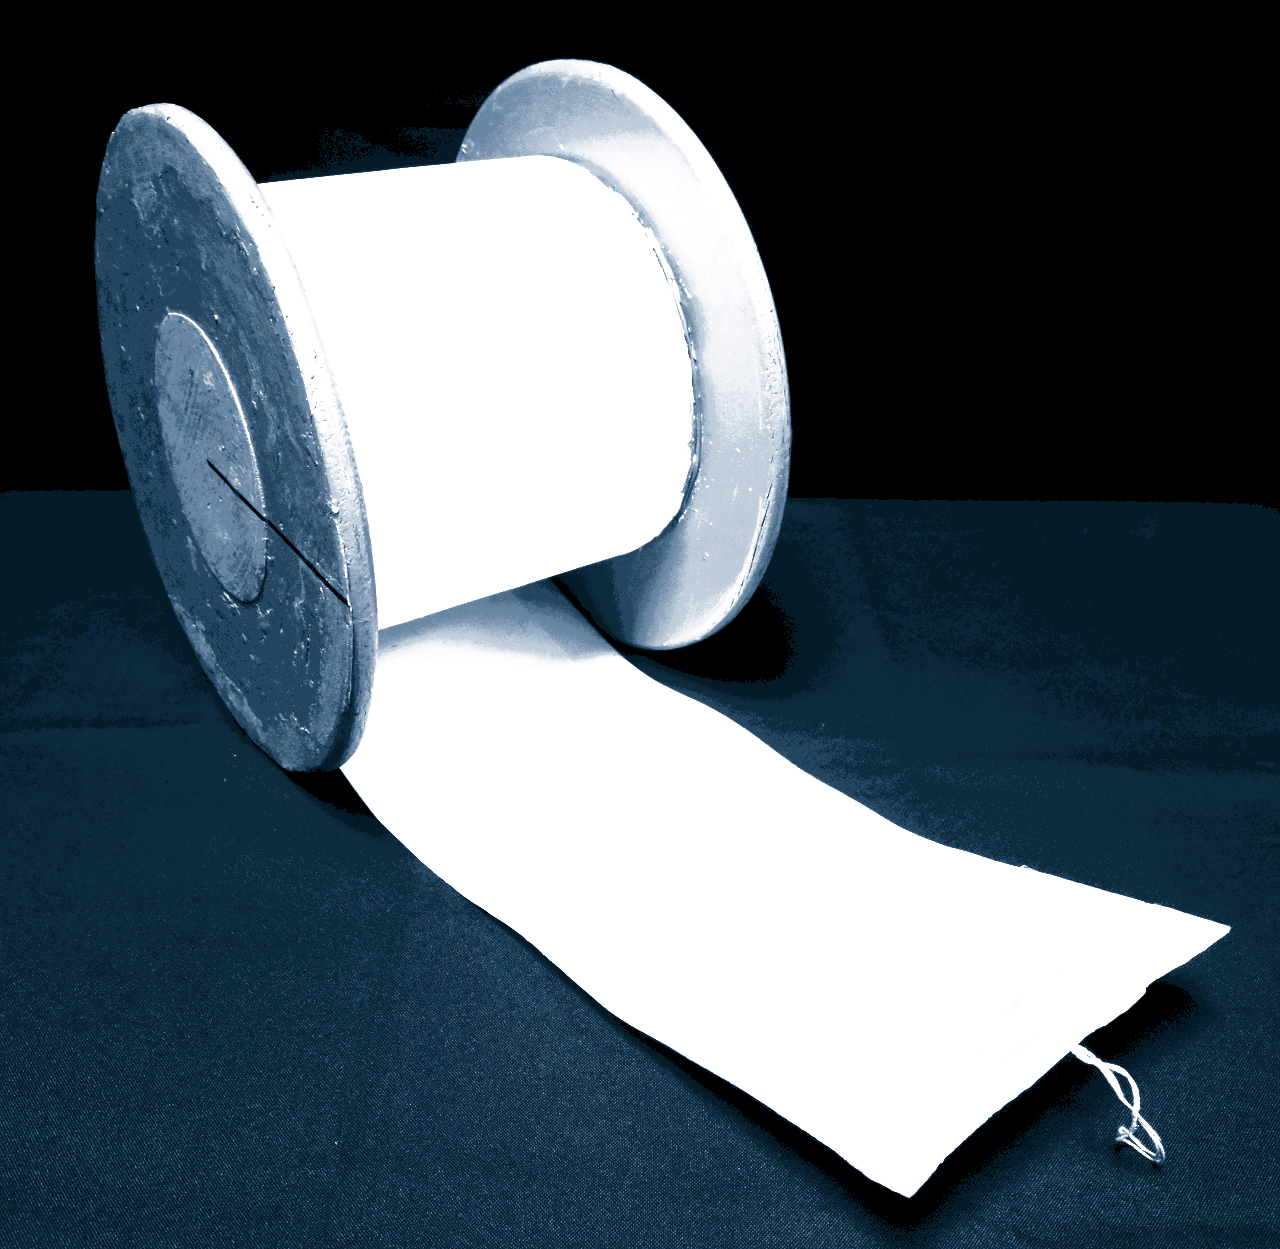
\includegraphics[width=0.75\linewidth]{roll-1.png}
	\caption{Демонстрация зависимости направления движения катушки от характера приложения силы}
	\label{roll-1}
\end{figure}

\subsection*{\textcolor{PineGreen}{Оборудование}}

\begin{enumerate}
	\item Катушка в виде оси с двумя дисками по краям.
	\item Нить или широкая полоска бумажного листа, намотанная на ось катушки.
\end{enumerate}

\subsection*{\textcolor{PineGreen}{Основные определения}}

При движении механической системы ее центр масс движется так, как двигалась бы материальная точка, имеющая массу, равную массе системы, и находящаяся под действием всех внешних сил, приложенных к системе. 
Кроме того, уравнение вращательного движения твердого тела по отношению к осям, проходящим через центр масс и движущимся вместе с ним поступательно, сохраняют тот же вид, что и для движения по отношению к инерциальной системе отсчета.
Ввиду этих свойств понятие о центре масс играет важную роль в динамике системы и твердого тела.

Тело находится в состоянии равновесия в поле силы тяжести, если каждая его точка остается все время неподвижной в некоторой инерциальной системе отсчета.
Условием равновесия материальной точки является равенство нулю равнодействующей (векторной суммы) всех сил, приложенных к точке.

Для тела конечного объема (система из материальных точек) важно учитывать точку приложения каждой силы.
Например, точка приложения вектора силы тяжести, действующего на тело вблизи поверхности Земли, называется центром тяжести.
Центр тяжести твердого тела в обычных условиях совпадает с центром масс.

Однако для твердого тела недостаточно потребовать равенства нулю векторной суммы всех приложенных к телу сил — необходимо учесть его способность вращаться:
\textit{\begin{flushleft}
		если тело обладает осью вращения и алгебраическая сумма моментов всех сил относительно этой оси обращается в нуль, то тело будет оставаться в равновесии.
\end{flushleft}}

\subsection*{\textcolor{PineGreen}{Краткое описание}}

Катушка представляет собой цилиндр из плотного картона, по краям которого расположены деревянные диски диаметром 200 мм.
К середине катушки прикрепляется конец широкой полоски бумаги, которая несколько раз оборачивается вокруг цилиндра.
Катушку кладут на стол и тянут за конец полоски, выходящий из-под нижней поверхности цилиндра. 
Катушка перемещается в ту или иную сторону в зависимости от того, какой момент силы больше относительно мгновенной оси $ O $, находящейся в плоскости стола: внешней силы \textit{F} или силы трения $ \textbf{F}_{\text{тр}} $.
В положении (\textit{а}) полоска бумаги закручивает катушку по часовой стрелке (рис.\ref{roll-2}), в положении (\textit{б}) — против.

\begin{figure}[H] 
	\centering 		
	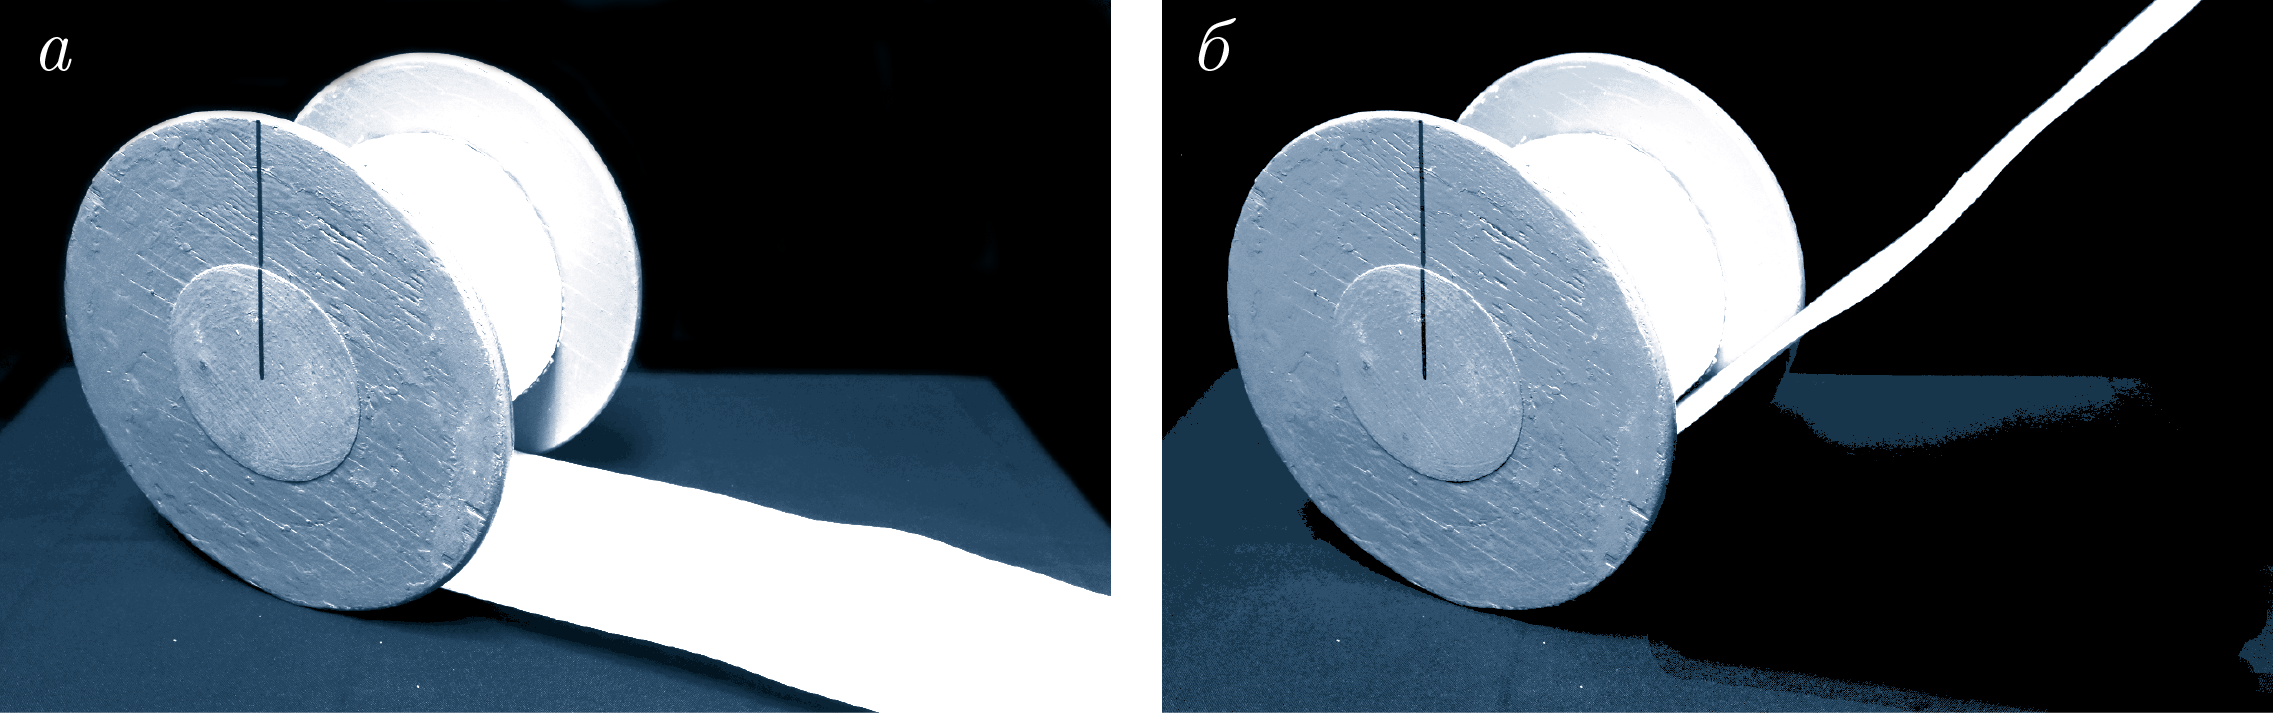
\includegraphics[width=0.9\linewidth]{roll-2.png} 
	\caption{В зависимости от способа приложения силы создаются моменты, вращающие катушку либо по ходу часовой стрелки (\textit{а}), либо против (\textit{б})}
	\label{roll-2}
\end{figure}

\subsection*{\textcolor{PineGreen}{Теория}}
Рассмотрим задачу о движении цилиндрического тела под действием силы \textit{F}, приложенной так, как показано на рис.\ref{roll-3}.

\begin{figure}[H] 
	\centering 		
	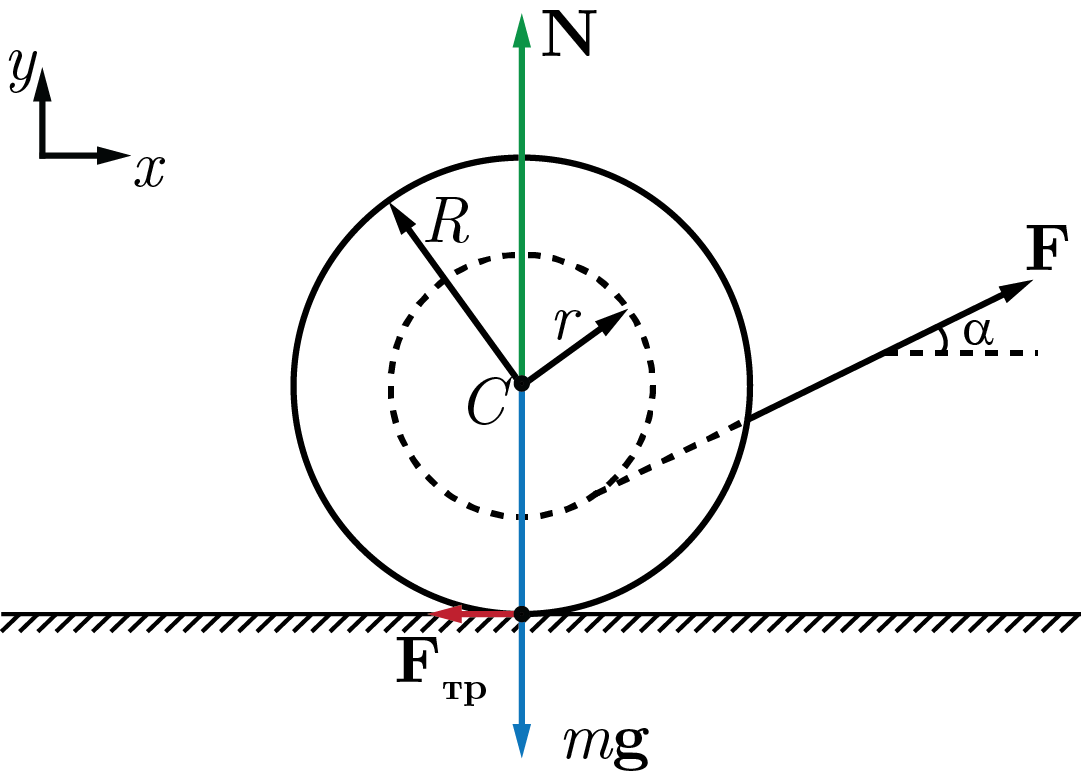
\includegraphics[width=0.6\linewidth]{roll-3.png} 
	\caption{Схематичное изображение катушки и действующих на нее сил}
	\label{roll-3}
\end{figure}

Запишем уравнение движения центра масс и основное уравнение динамики вращательного движения:
\begin{equation}\label{roll-eq1}
\begin{cases}
\textbf{F} + \textbf{F}_{\text{тр}} = m\textbf{a} \\
\textbf{M}_{F\text{тр}} + \textbf{M}_F= I\textbf{ε},
\end{cases}
\end{equation}
где \textit{m} — масса катушки, \textbf{a} — вектор поступательного ускорения точек тела, \textit{I} — момент инерции катушки относительно оси, проходящей вдоль ее оси, \textbf{ε} — вектор углового ускорения тела, создаваемый моментом $ \textbf{M}_F $ внешней силы, $ \textbf{M}_{\text{Fтр}} $ — момент силы трения.

Уравнения записанной выше системы необходимо спроецировать на соответствующие координатные оси:

\begin{equation}\label{roll-eq2}
\begin{cases}
Ox: F\cos\alpha - F_{\text{тр}} = ma \\
Oz: F_{\text{тр}}R - Fr= I \varepsilon.
\end{cases}
\end{equation}

Пользуясь известным соотношением между линейным и угловым ускорением ($ a = \varepsilon R $), можно из первого уравнения системы выразить силу трения $  F_{\text{тр}} = F\cos\alpha - m  \varepsilon R $ и подставить во второе уравнение:
\begin{equation}\label{roll-eq3}
F R \cos\alpha - m  \varepsilon R^{2} - Fr= I \varepsilon.
\end{equation}
\begin{equation}\label{roll-eq4}
 \varepsilon (I  + mR^{2})  = F (R \cos \alpha - r).
\end{equation}

После этого можно получить выражение для углового ускорения $ \varepsilon $:
\begin{equation}\label{roll-eq5}
\varepsilon = \frac{F(R \cos \alpha - r)}{(I  + mR^{2})}
\end{equation}

Затем, используя это соотношение, можно выразить линейное ускорение $ a $:
\begin{equation}\label{roll-eq6}
a = \varepsilon R = \frac{FR(R \cos \alpha - r)}{(I + mR^{2})}.
\end{equation}

Из полученного уравнения видно, что для случая $ a<0 $ (движение в сторону, противоположную направлению силы \textbf{F}), необходимо чтобы выполнялось следующее условие: $ \cos \alpha < r/R$. Такая ситуация возникает, когда внешняя сила \textbf{F} направлена под достаточно крутым углом к горизонту.

Стоит отметь, что момент инерции складывается из моментов инерции втулки и двух крайних дисков (рис.\ref{roll-2}).
Его значение можно либо взять из таблицы, либо определить опытным путем.  

\end{document}
